\documentclass[12pt]{article}

\usepackage{sbc-template}
\usepackage{graphicx,url}
\usepackage[utf8]{inputenc}
\usepackage{booktabs}
\usepackage{amsmath}

% Rótulos em português (sem babel: pacote de idioma indisponível no ambiente)
\renewcommand{\figurename}{Figura}
\renewcommand{\tablename}{Tabela}
\renewcommand{\refname}{Referências}

\sloppy

\title{RECLin-PT: Extração de Relações em Notas Clínicas em Português sobre o
Corpus SemClinBr}

\author{Angelo A. L. Silveira Filho\inst{1} \and Cristiano da Silveira
Colombo\inst{1}}

\address{Bacharelado em Sistemas de Informação\\
  Instituto Federal de Educação, Ciência e Tecnologia do Espírito Santo (IFES)\\
  Cachoeiro de Itapemirim -- ES -- Brasil
  \email{angelo.silveira@aluno.ifes.edu.br \quad cristiano.colombo@ifes.edu.br}
}

\begin{document}

\maketitle

\begin{abstract}
Clinical free text concentrates information whose interpretation depends on the
relation between concepts, particularly the negation of findings. As the initial
stage of developing \textbf{RECLin-PT} --- an improved clinical relation
extraction (RE) model for Portuguese --- this work reports the baseline results
that ground that development. We fine-tune two Portuguese encoders under an
identical experimental pipeline (the supporting infrastructure, not a named
model): a clinical-domain one (BioBERTpt) and a general-domain one (BERTimbau),
over the SemClinBr corpus in a three-class space (negation, association and
no-relation), changing only the pre-trained checkpoint. On the frozen test set,
the two baselines are statistically tied on the \texttt{negation\_of} F1 (0.724
vs.\ 0.734; McNemar $p=0.18$; paired bootstrap 95\% CI $[-0.047,+0.026]$), and
the seed-to-seed variation exceeds the gap between them. These initial results
indicate that RECLin-PT can be built upon the best-performing baseline, with no
significant penalty from adopting the more efficient general encoder.
\end{abstract}

\begin{resumo}
O texto clínico livre concentra informação cuja interpretação depende da relação
entre conceitos, em especial a negação de achados. Como etapa inicial do
desenvolvimento do \textbf{RECLin-PT} --- um modelo aprimorado de extração de
relações (\emph{Relation Extraction}, RE) clínicas em português ---, este
trabalho apresenta os resultados dos \emph{baselines} que fundamentam esse
desenvolvimento. Ajustamos dois \emph{encoders} para o português sob uma mesma
infraestrutura experimental, um de domínio clínico (BioBERTpt) e um de domínio
geral (BERTimbau), sobre o corpus SemClinBr, em um espaço de três classes
(negação, associação e ausência de relação), variando apenas o \emph{checkpoint}
de pré-treino. No conjunto de teste congelado, os dois \emph{baselines} empatam
estatisticamente no F1 de \texttt{negation\_of} (0,724 vs.\ 0,734; McNemar
$p=0,18$; \emph{bootstrap} pareado IC95\% $[-0,047;+0,026]$), e a variação entre
sementes supera a diferença entre eles. Esses resultados iniciais indicam que o
RECLin-PT pode ser construído a partir do melhor \emph{baseline}, sem penalidade
significativa ao adotar o \emph{encoder} geral, mais eficiente.
\end{resumo}

\section{Introdução}

O registro eletrônico em saúde concentra grande parte da informação clínica sob
a forma de texto livre. Notas de evolução, sumários de alta e laudos são
redigidos em linguagem natural, com abreviações idiossincráticas, ausência
frequente de pontuação padronizada e construções negativas características do
discurso médico. Essa riqueza textual, embora valiosa para pesquisa e apoio à
decisão, permanece majoritariamente inacessível a consultas estruturadas, o que
motiva o desenvolvimento de técnicas de Processamento de Linguagem Natural (PLN)
capazes de transformar texto clínico em conhecimento estruturado.

O reconhecimento de entidades nomeadas identifica menções a conceitos clínicos
(sintomas, doenças, achados, procedimentos), mas isoladamente não captura como
esses conceitos se articulam no enunciado. Saber que um documento menciona
``febre'' não é suficiente: é preciso distinguir se a febre está associada ao
quadro do paciente ou se está sendo negada (``paciente afebril''). Esse vínculo
é o objeto da extração de relações (\emph{Relation Extraction}, RE), modelada
aqui como a classificação de um par ordenado de entidades $(e_1, e_2)$ dentro do
espaço de rótulos \texttt{negation\_of}, \texttt{associated\_with} e
\texttt{no\_relation}.

A negação clínica é um fenômeno linguístico de alto impacto: tratar um achado
negado como presente pode inverter completamente a interpretação de um
prontuário. Em português, a negação é fortemente lexicalizada (``não'', ``sem'',
``nega'', ``ausência de''), e há a expectativa difundida de que modelos
pré-treinados sobre texto do próprio domínio clínico capturem melhor essas
construções do que modelos de domínio geral. Essa expectativa, contudo, é
raramente testada de forma controlada para o português: trabalhos costumam adotar
um modelo clínico por hipótese, sem isolar o efeito do pré-treinamento de
domínio sob protocolo estatístico rigoroso.

Este trabalho integra o desenvolvimento do \textbf{RECLin-PT}, um modelo
aprimorado de extração de relações em texto clínico em português sobre o corpus
SemClinBr. Como etapa inicial dessa construção, conduz-se um experimento
controlado de \emph{baselines} para responder a uma questão fundamental que
fundamenta as decisões de projeto seguintes: \textbf{o pré-treinamento clínico
importa para a extração de relações em textos médicos em português?} Para
respondê-la, comparam-se dois \emph{encoders} para o português na \emph{mesma}
tarefa de RE sobre o SemClinBr~\cite{oliveira:22}, mudando \emph{somente} o
\emph{checkpoint} de pré-treino: o BioBERTpt~\cite{schneider:20}, adaptado a
narrativas clínicas e biomédicas em português, e o BERTimbau~\cite{souza:20},
pré-treinado em texto de domínio geral (brWaC). Ambos são ajustados sob uma única
cadeia determinística, compartilhando a representação de entrada, a função de
perda, o escalonador, a seleção de modelo, as métricas e a semente, de modo que
qualquer diferença observada possa ser atribuída ao pré-treinamento, e não a
artefatos de implementação. O RECLin-PT será, então, desenvolvido a partir do
\emph{encoder} que se mostrar a melhor base nesses \emph{baselines}.

As contribuições iniciais deste trabalho são: (i) uma infraestrutura
experimental reprodutível e controlada --- do texto bruto às métricas finais ---
que viabiliza a comparação justa de \emph{baselines} para o desenvolvimento do
RECLin-PT; (ii) uma comparação empírica, com teste de significância pareado,
entre um \emph{encoder} clínico e um geral sobre o SemClinBr; e (iii) a
identificação da melhor base sobre a qual construir o RECLin-PT, observando que o
\emph{encoder} de domínio geral iguala estatisticamente o clínico, inclusive na
classe de negação, com cerca de 60\% dos parâmetros. O restante do trabalho está
organizado da seguinte forma: a Seção~\ref{sec:fund} apresenta a fundamentação
teórica; a Seção~\ref{sec:met} detalha a metodologia; a Seção~\ref{sec:res}
reporta os resultados iniciais dos \emph{baselines}; e a
Seção~\ref{sec:conc} traz as considerações parciais.

\subsection{Trabalhos relacionados}
A extração de relações clínicas consolidou-se em língua inglesa em torno de
campanhas de avaliação como as séries i2b2 e n2c2~\cite{uzuner:11}, que
disponibilizaram corpora anotados e tarefas compartilhadas para problemas como
relações entre medicamentos, dosagens e efeitos adversos. Esses esforços
estabeleceram protocolos de avaliação e evidenciaram a importância de tratar
adequadamente o desbalanceamento de classes e o vazamento de dados entre
partições --- preocupações transpostas para este trabalho. No plano dos modelos,
o BioBERT~\cite{lee:20} demonstrou ganhos da adaptação de domínio biomédico em
inglês, e técnicas de representação de pares por marcadores de
entidade~\cite{soares:19} tornaram-se padrão para RE com modelos baseados em
BERT.

O desenvolvimento de PLN clínico em português foi por muito tempo limitado pela
ausência de corpora anotados de acesso controlado. O SemClinBr~\cite{oliveira:22}
preencheu parte dessa lacuna ao disponibilizar mil documentos clínicos anotados
semanticamente, acompanhados de dicionários de abreviações e de pistas de
negação. No plano dos modelos, o BioBERTpt~\cite{schneider:20} adaptou o
paradigma de modelos contextuais ao domínio clínico em português, demonstrando
ganhos em reconhecimento de entidades nomeadas em relação a modelos de domínio
geral; o BERTimbau~\cite{souza:20}, por sua vez, é a referência de domínio geral
para o português. Enquanto boa parte da literatura em português concentra-se em
NER e adota um modelo clínico por hipótese, o RECLin-PT aborda a etapa subsequente
de RE e, como ponto de partida, \emph{testa} de forma controlada se o ganho do
pré-treinamento clínico observado em NER se transfere para a extração de relações,
com atenção particular à negação clínica.

\section{Fundamentação Teórica}\label{sec:fund}

\subsection{Processamento de linguagem natural clínico}
O PLN clínico ocupa-se da análise automática de textos produzidos no cuidado em
saúde. Esses textos apresentam características que os distinguem da linguagem
geral: vocabulário técnico, abreviações não padronizadas, telegrafismo (omissão
de elementos gramaticais) e prevalência de construções negativas e de incerteza.
Tais propriedades tornam a transferência direta de ferramentas treinadas em
domínio aberto pouco eficaz, motivando recursos e modelos específicos do
domínio --- hipótese cuja validade, para a tarefa de RE em português, é
justamente a questão que orienta esta etapa inicial do trabalho.

\subsection{Extração de relações}
A extração de informação em texto clínico costuma ser decomposta em duas tarefas
encadeadas. A primeira, o reconhecimento de entidades nomeadas, delimita trechos
do texto que mencionam conceitos de interesse e lhes atribui um tipo semântico.
A segunda, a RE, determina se um par de entidades mantém uma relação e de que
tipo. Formalmente, dado um par ordenado $(e_1, e_2)$ em um documento, a RE é
modelada como um problema de classificação que associa ao par um rótulo dentro
de um conjunto pré-definido. Neste trabalho o espaço de rótulos é
\texttt{negation\_of}, \texttt{associated\_with} e \texttt{no\_relation}. O
rótulo \texttt{no\_relation} é fundamental: como a anotação de corpora registra
apenas relações positivas, todo par de entidades não anotado deve ser tratado
como ausência de relação, o que introduz um forte desbalanceamento de classes.

\subsection{A negação clínica}
Em detecção de negação clínica, o algoritmo NegEx~\cite{chapman:01} tornou-se
referência: a partir de um léxico de gatilhos de negação e de janelas de
contexto, classifica achados como negados ou afirmados. Sua eficácia deriva do
fato de a negação clínica ser altamente lexicalizada. Em português, gatilhos
como ``não'', ``sem'', ``nega'' e ``ausência de'', além de adjetivos que embutem
negação morfologicamente (``afebril'', ``anictérico''), sustentam estratégias
análogas. A alta lexicalização sugere que o sinal de negação possa estar
acessível mesmo a modelos não especializados no domínio, o que torna a
comparação entre \emph{encoders} clínico e geral particularmente informativa.

\subsection{Modelos baseados em \emph{Transformers}}
A arquitetura \emph{Transformer}~\cite{vaswani:17}, baseada em mecanismos de
atenção, viabilizou modelos de linguagem pré-treinados que produzem
representações contextuais das palavras. O BERT~\cite{devlin:19} popularizou o
paradigma de pré-treinamento seguido de ajuste fino (\emph{fine-tuning}) para
tarefas específicas. Para o português, há tanto modelos de domínio geral, como o
BERTimbau~\cite{souza:20}, pré-treinado no corpus brWaC, quanto modelos de
domínio clínico, como o BioBERTpt~\cite{schneider:20}, adaptado a narrativas
clínicas e biomédicas em português brasileiro. Esses dois modelos compartilham a
mesma arquitetura base (BERT) e diferem essencialmente no corpus de
pré-treinamento, o que os torna candidatos naturais a um experimento controlado
sobre a importância do domínio de pré-treino.

\section{Metodologia}\label{sec:met}

Os dois \emph{encoders} avaliados --- BioBERTpt e BERTimbau --- são tratados como
\emph{baselines}, comparados para identificar a melhor base sobre a qual o
RECLin-PT será desenvolvido. A infraestrutura experimental descrita a seguir não
constitui um modelo com nome próprio: é apenas a cadeia que viabiliza essa
comparação de forma justa e reprodutível. A premissa metodológica central é a
\emph{paridade}: os dois \emph{baselines} compartilham um único núcleo de
implementação e diferem apenas no \emph{checkpoint} de pré-treino. Todas as
etapas foram projetadas sob reprodutibilidade: ordenação determinística das
saídas, serialização fixa e semente aleatória registrada (42).

\subsection{Corpus SemClinBr e representação canônica}
Utiliza-se o corpus SemClinBr~\cite{oliveira:22}, composto por mil documentos
clínicos em português anotados com entidades e relações, distribuído sob licença
restrita. Um \emph{parser} determinístico converte cada arquivo XML em um
registro canônico no formato JSONL, com identificador do documento, texto, lista
de entidades (tipo e \emph{offsets}) e lista de relações. O \emph{parser} é fiel
ao XML e executa verificações de sanidade (correspondência entre o texto
extraído por \emph{offset} e o atributo anotado, validade dos intervalos e
integridade referencial das relações), corrigindo automaticamente pequenos
deslocamentos de \emph{offset} ($\pm1$ e $\pm2$ caracteres) e acumulando as
inconsistências em um log de avisos.

A análise da representação canônica totaliza 1.000 documentos, 45.508 entidades
(média de 45,5 por documento) e 11.458 relações (média de 11,5; mediana de 10;
máximo de 65 por documento); 46 documentos (4,60\%) não possuem relação anotada.
As relações distribuem-se de forma fortemente desbalanceada entre os dois tipos
anotados: \texttt{associated\_with} responde por 9.852 ocorrências (86,0\%) e
\texttt{negation\_of} por 1.606 (14,0\%). Esse desequilíbrio motiva tanto a
escolha do macro-F1 como métrica principal quanto o tratamento explícito de
classes no ajuste dos \emph{baselines}.

\subsection{Particionamento dos dados}
A partição segue a razão 80/10/10 em nível de \emph{documento}, e não de relação.
Essa escolha previne o vazamento de dados: relações de um mesmo documento
compartilham vocabulário e trechos repetidos, e dividi-las entre partições
diferentes inflaria artificialmente as métricas de teste. A partição é
estratificada pela presença das classes \texttt{negation\_of} e
\texttt{associated\_with} em cada documento, por meio do algoritmo de
estratificação multirrótulo de~\cite{sechidis:11}, de modo a garantir
representação estável da classe minoritária. A partição é gerada com semente fixa
(42) e congelada. O resultado são 800 documentos de treino, 100 de
desenvolvimento e 100 de teste; a proporção de \texttt{negation\_of} permanece
estável (entre 13,7\% e 15,0\%) em todas as partições, condição necessária para
que a estimativa de F1 dessa classe no teste seja confiável.

\subsection{Geração de pares candidatos}
O SemClinBr anota apenas relações positivas. Avaliar um classificador no espaço
\{\texttt{negation\_of}, \texttt{associated\_with}, \texttt{no\_relation}\} exige,
portanto, construir os exemplos negativos. A geração é feita por uma função
compartilhada por ambos os \emph{baselines} --- condição necessária para que os
resultados fiquem na mesma régua estatística. Para cada documento, percorrem-se
todos os pares ordenados de entidades $(e_1, e_2)$, $e_1 \neq e_2$ (a ordem
importa, porque a direção é relevante para a negação); descartam-se os pares cuja
distância exceda a janela máxima ($\texttt{max\_gap}=20$) e os pares entre
documentos distintos; e atribui-se o rótulo: se o par ordenado coincide com uma
relação anotada, recebe o tipo \emph{gold}; caso contrário, recebe
\texttt{no\_relation}. A emissão segue ordenação determinística, de modo que o
conjunto de candidatos e o \emph{hash} das predições sejam estáveis entre
execuções.

O procedimento gera 128.380 candidatos de treino, 15.994 de desenvolvimento e
16.074 de teste. A consequência é um conjunto de teste fortemente desbalanceado:
a classe \texttt{no\_relation} concentra 14.959 instâncias (93,1\%), enquanto
\texttt{associated\_with} e \texttt{negation\_of} somam, respectivamente, 964 e
151. A janela impõe um teto de \emph{recall}: relações cujo par fique além de
\texttt{max\_gap} jamais são geradas como candidato. No teste, esse limite é
desprezível para a negação (151 de 152 relações \emph{gold} preservadas), mas
mais sensível para \texttt{associated\_with}, fixando um teto de \emph{recall}
documentado para essa classe. Como ambos os \emph{baselines} recebem exatamente
os mesmos candidatos, o teto é idêntico para os dois e não afeta a comparação.

\subsection{Representação de entrada: marcadores tipados e grupos UMLS}
Cada par candidato é transformado na \emph{string} de entrada do \emph{encoder}
com marcadores de entidade tipados, no esquema
\texttt{[E1] <grupo> : superfície [/E1] $\ldots$ [E2] <grupo> : superfície
[/E2]}. Os quatro marcadores são registrados como \emph{tokens} especiais no
\emph{tokenizer}, a ordem $(e_1, e_2)$ preserva a direção da relação, e a
representação do par alimentada ao cabeçote de classificação é a concatenação dos
estados ocultos dos marcadores de início, na linha de~\cite{soares:19}.

O campo \texttt{<grupo>} não é o tipo bruto da entidade. O SemClinBr anota cada
entidade com tipos semânticos da UMLS, frequentemente em rótulos múltiplos
separados por ``\texttt{|}'' (por exemplo, \texttt{Medical Device|Finding|%
Abbreviation}). Usar a \emph{string} de tipo diretamente faria o número de
símbolos distintos explodir (centenas de combinações mal povoadas no treino),
prejudicando a generalização. A solução agrega os tipos atômicos nos 15 grupos
semânticos da UMLS~\cite{mccray:01} --- por exemplo, \texttt{DISO} (transtornos),
\texttt{CHEM} (químicos e fármacos), \texttt{PROC} (procedimentos) ---,
acrescidos de duas camadas próprias do corpus que carregam sinal relevante para a
tarefa: \texttt{Abbreviation} e \texttt{Negation} (esta diretamente associada à
classe \texttt{negation\_of}). Como a mesma representação de entrada é aplicada
aos dois \emph{baselines}, qualquer efeito dessa escolha é compartilhado e não
confunde a comparação.

\subsection{Baselines comparados e paridade}
Comparam-se dois \emph{encoders} para o português, tratados como \emph{baselines}
sob a mesma tarefa, variando apenas o \emph{checkpoint} de pré-treino:
\begin{itemize}
  \item \textbf{BioBERTpt} (\texttt{pucpr/biobertpt-all}) --- \emph{encoder} de
  domínio \emph{clínico}, com 177,9 milhões de parâmetros~\cite{schneider:20}.
  \item \textbf{BERTimbau} (\texttt{neuralmind/bert-base-portuguese-cased}) ---
  \emph{encoder} de domínio \emph{geral}, pré-treinado no brWaC, com 108,9
  milhões de parâmetros~\cite{souza:20}.
\end{itemize}
Os dois compartilham um único núcleo de implementação e, portanto, são idênticos
por construção em tudo, exceto o modelo: a representação de entrada por
marcadores tipados; a perda de entropia cruzada com
\texttt{class\_weight="balanced"}, que reescala o erro de forma inversamente
proporcional à frequência de cada classe (sem o que o otimizador minimizaria o
erro prevendo \texttt{no\_relation} para quase tudo); o escalonador linear com
\emph{warmup}; a seleção da melhor época pelo macro-F1 no conjunto de
desenvolvimento; e a semente de reprodutibilidade (42). Trocar um \emph{baseline}
pelo outro consiste apenas em mudar o \emph{checkpoint} carregado. O melhor
\emph{baseline} identificado por esse protocolo será a base do RECLin-PT.

\subsection{Protocolo de avaliação}
A métrica principal é o macro-F1, que atribui peso igual às três classes e,
portanto, penaliza modelos que ignoram as classes minoritárias --- comportamento
desejável dado o desbalanceamento. Classes ausentes nas predições recebem F1
nulo, conforme~\cite{forman:10}. Reportam-se também o F1 por classe, o micro-F1
(acurácia), o \emph{weighted}-F1 e o coeficiente de correlação de Matthews
(MCC), robusto a desbalanceamento. A métrica que responde diretamente à pergunta
``o modelo detecta bem a negação?'' é o F1 de \texttt{negation\_of} no teste.

A comparação entre os dois \emph{baselines} emprega dois testes complementares,
calculados sobre o mesmo conjunto de teste a partir das predições salvas. O teste
de McNemar~\cite{dietterich:98} olha apenas os casos em que os modelos discordam
no acerto ($b$ = o primeiro acerta e o segundo erra; $c$ = o inverso) e, sob a
hipótese nula de mesma taxa de acerto, avalia $b \sim \mathrm{Binomial}(b+c,
0{,}5)$ pelo teste binomial exato; mede se os padrões de erro globais diferem.
O \emph{bootstrap} pareado no F1 de \texttt{negation\_of} reamostra os exemplos
do teste com reposição 10.000 vezes e recalcula a diferença $F1_A - F1_B$,
reportando a diferença média, o intervalo de confiança de 95\% (percentis
2,5/97,5) e um valor-$p$ bilateral; mede diretamente se a vantagem na negação é
robusta. Como análise de robustez à variação de inicialização, o BioBERTpt é
treinado também com uma segunda semente (43).

\subsection{Ambiente experimental}
O ajuste fino é executado em GPU (Google Colab, Tesla T4); o parsing, o
particionamento, a geração de candidatos e os testes de significância executam em
CPU. Os principais hiperparâmetros são: \texttt{max\_length} de 128
\emph{tokens}, janela de contexto de 128 caracteres em torno do par, tamanho de
lote 64, taxa de aprendizado $2\times10^{-5}$ (AdamW), 3 épocas e seleção de
modelo por macro-F1 no desenvolvimento. Esses valores são idênticos para os dois
\emph{baselines}.

\section{Resultados Iniciais}\label{sec:res}

Esta seção reporta os resultados iniciais dos \emph{baselines}, que orientarão o
desenvolvimento do RECLin-PT. Todos os modelos foram avaliados sobre o mesmo
conjunto de teste, composto por 16.074 pares candidatos (14.959
\texttt{no\_relation}, 964 \texttt{associated\_with} e 151
\texttt{negation\_of}). A Tabela~\ref{tab:resultados} consolida os resultados dos
dois \emph{baselines} na semente 42. Os melhores valores por coluna estão em
negrito.

\begin{table}[ht]
\centering
\caption{Resultados dos \emph{baselines} no conjunto de teste (semente 42).
Negrito indica o melhor valor por coluna.}
\label{tab:resultados}
\begin{tabular}{lcccccc}
\toprule
\textbf{Baseline} & \textbf{Macro-F1} & \textbf{F1 neg.} & \textbf{F1 assoc.} &
\textbf{F1 no\_rel.} & \textbf{MCC} & \textbf{Acur.} \\
\midrule
BioBERTpt (clínico) & \textbf{0,707} & 0,724 & \textbf{0,460} &
\textbf{0,935} & \textbf{0,487} & \textbf{0,885} \\
BERTimbau (geral)   & 0,704 & \textbf{0,734} & 0,445 & 0,934 & 0,471 & 0,882 \\
\bottomrule
\end{tabular}
\end{table}

\subsection{Desempenho dos dois \emph{baselines}}
Os dois \emph{baselines} apresentam desempenho praticamente indistinguível. O
BioBERTpt clínico atinge macro-F1 de 0,707 e o BERTimbau geral, 0,704 --- uma
diferença de 0,003. Na métrica-alvo, o F1 de \texttt{negation\_of}, a ordem
inclusive se inverte: o BERTimbau geral (0,734) supera marginalmente o BioBERTpt
clínico (0,724). As demais métricas seguem o mesmo padrão de quase empate: ambos
alcançam \emph{recall} alto na negação (BioBERTpt 0,894; BERTimbau 0,887) com
precisão moderada ($\approx$0,61--0,63), e ambos têm na classe
\texttt{associated\_with} a maior dificuldade (F1 $\approx$0,45--0,46), com alta
cobertura mas baixa precisão, refletindo a dificuldade de distinguir associação
genuína de mera proximidade textual. A Figura~\ref{fig:f1classe} resume o F1 por
classe dos dois \emph{baselines}.

\begin{figure}[ht]
\centering
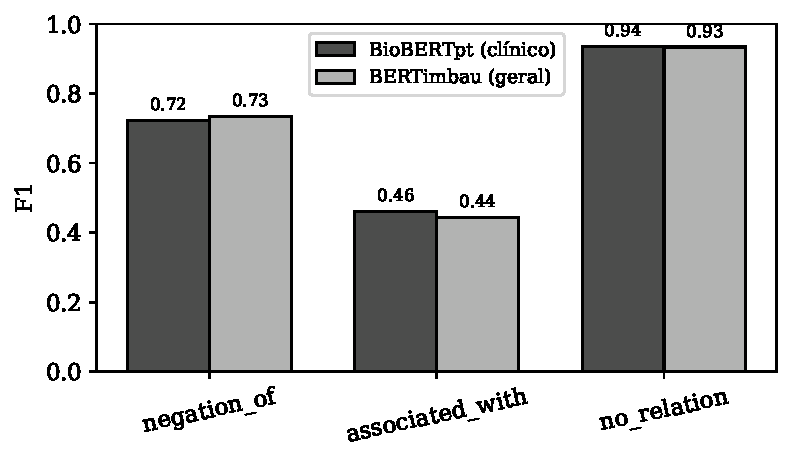
\includegraphics[width=.72\textwidth]{figs/f1_por_classe.pdf}
\caption{F1 por classe no conjunto de teste: BioBERTpt (clínico) vs.\ BERTimbau
(geral). As barras são praticamente coincidentes em todas as classes.}
\label{fig:f1classe}
\end{figure}

\subsection{Matrizes de confusão}
As Figuras~\ref{fig:cmbio} e~\ref{fig:cmber} apresentam as matrizes de confusão
dos dois \emph{baselines}, normalizadas por linha (cada célula é a fração das
instâncias de uma classe verdadeira atribuída a cada classe predita; a diagonal
corresponde ao \emph{recall} por classe). Os dois padrões de erro são
notavelmente semelhantes: diagonal forte na negação e na classe majoritária, e o
erro dominante remanescente na confusão entre \texttt{associated\_with} e
\texttt{no\_relation} --- coerente com a baixa precisão daquela classe nos dois
modelos. A semelhança qualitativa entre as matrizes reforça a leitura de que os
dois \emph{encoders} aprendem essencialmente a mesma função para esta tarefa.

\begin{figure}[ht]
\centering
\begin{minipage}{.49\textwidth}
  \centering
  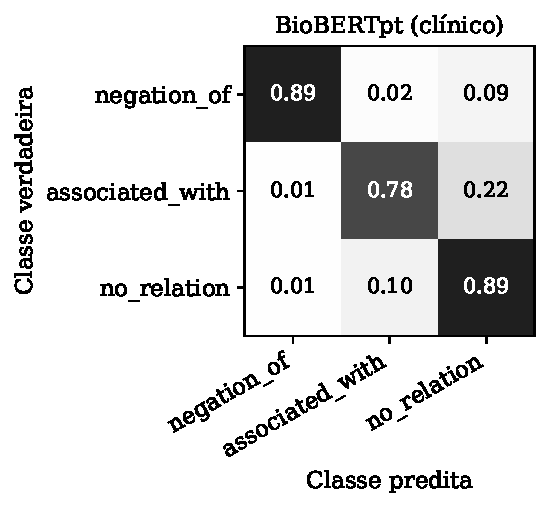
\includegraphics[width=\textwidth]{figs/cm_biobertpt.pdf}
  \caption{Matriz de confusão do BioBERTpt (clínico), normalizada por linha.}
  \label{fig:cmbio}
\end{minipage}\hfill
\begin{minipage}{.49\textwidth}
  \centering
  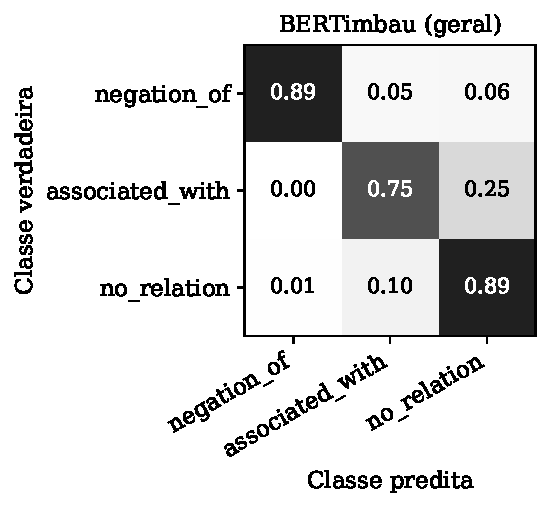
\includegraphics[width=\textwidth]{figs/cm_bertimbau.pdf}
  \caption{Matriz de confusão do BERTimbau (geral), normalizada por linha.}
  \label{fig:cmber}
\end{minipage}
\end{figure}

\subsection{Significância estatística}
A proximidade dos valores pontuais sugere empate, mas a conclusão exige um teste
pareado. A Tabela~\ref{tab:signif} reporta a comparação direta entre os dois
\emph{baselines} no conjunto de teste. No F1 de \texttt{negation\_of}, a
diferença observada é de apenas $-0,010$ (a favor do BERTimbau geral). O teste de
McNemar não rejeita a hipótese nula de igualdade ($p=0,18$): das 946 instâncias
em que os modelos discordam, 494 favorecem o BioBERTpt e 452 o BERTimbau, uma
assimetria compatível com o acaso. O \emph{bootstrap} pareado confirma o
resultado: o intervalo de confiança de 95\% para a diferença no F1 de
\texttt{negation\_of} é $[-0,047;+0,026]$, que \emph{inclui o zero}, com
valor-$p$ de 0,57. Em ambos os testes, portanto, \textbf{não há diferença
estatisticamente significativa} entre o \emph{encoder} clínico e o geral.

\begin{table}[ht]
\centering
\caption{Comparação pareada BioBERTpt (clínico) vs.\ BERTimbau (geral) no teste
($n=16.074$, semente 42).}
\label{tab:signif}
\begin{tabular}{lc}
\toprule
\textbf{Medida} & \textbf{Valor} \\
\midrule
F1 \texttt{negation\_of} --- BioBERTpt (A) & 0,724 \\
F1 \texttt{negation\_of} --- BERTimbau (B) & 0,734 \\
Diferença observada (A $-$ B) & $-0,010$ \\
McNemar: $b$ (só A acerta) / $c$ (só B acerta) & 494 / 452 \\
McNemar: valor-$p$ (binomial exato) & 0,18 \\
\emph{Bootstrap} pareado: IC95\% da diferença & $[-0,047;\,+0,026]$ \\
\emph{Bootstrap} pareado: valor-$p$ & 0,57 \\
\textbf{Diferença significativa ($\alpha=0,05$)?} & \textbf{Não} \\
\bottomrule
\end{tabular}
\end{table}

\subsection{Robustez à semente}
Para situar a magnitude da diferença entre os \emph{baselines}, treinamos o
BioBERTpt com uma segunda semente (43). O macro-F1 cai de 0,707 (semente 42) para
0,665 (semente 43), e o F1 de \texttt{negation\_of}, de 0,724 para 0,653 --- uma
variação de 0,071 atribuível \emph{apenas} à inicialização aleatória do treino.
Essa variação entre sementes de um \emph{mesmo} modelo é cerca de sete vezes
maior que a diferença de 0,010 observada entre o BioBERTpt e o BERTimbau na
semente 42. Em outras palavras, o ruído de treino do \emph{encoder} clínico,
isoladamente, é maior que a vantagem que se poderia atribuir ao domínio de
pré-treino, o que reforça a leitura de empate.

\subsection{Análise dos resultados}
O resultado central é um \emph{empate estatístico}: para a extração de relações
no SemClinBr, no espaço de três classes, o pré-treinamento clínico do BioBERTpt
não produz vantagem mensurável sobre o pré-treinamento geral do BERTimbau, nem
mesmo na classe de negação, onde a especialização de domínio seria mais
plausível. Esse achado contrasta com a expectativa difundida --- e com os ganhos
relatados para NER clínico em português~\cite{schneider:20} --- de que modelos de
domínio sempre se transfiram melhor.

Duas explicações são plausíveis e compatíveis com os dados. Primeiro, a negação
clínica em português é fortemente lexicalizada (``não'', ``sem'', ``nega'',
``afebril''); esse sinal é frequente e regular o bastante para que um
\emph{encoder} de domínio geral, com vocabulário amplo do português, o capture
tão bem quanto um clínico, sobretudo quando reforçado pelos marcadores tipados de
entrada e pela camada \texttt{Negation} dos grupos UMLS. Segundo, a tarefa, tal
como formulada, depende mais da estrutura local do par (direção, proximidade,
tipos semânticos das entidades) do que de conhecimento lexical especializado de
domínio, e essa estrutura é fornecida igualmente aos dois \emph{baselines} pela
representação de entrada compartilhada.

Um corolário prático --- e diretamente relevante para o desenvolvimento do
RECLin-PT --- é a eficiência: o BERTimbau iguala o BioBERTpt com aproximadamente
60\% dos parâmetros (108,9 vs.\ 177,9 milhões). Quando o desempenho é
equivalente, o modelo menor é preferível por custo de inferência e de memória ---
uma consideração concreta para implantação em ambientes clínicos com recursos
limitados, e um argumento a favor de construir o RECLin-PT sobre o \emph{encoder}
geral.

\subsection{Limitações e ameaças à validade}
Quanto à validade interna, o congelamento das partições com semente fixa e o
particionamento em nível de documento mitigam o vazamento de dados, a principal
causa de resultados não reproduzíveis em PLN biomédico; e a paridade total de
implementação entre os dois \emph{baselines} garante que a diferença medida
reflita o \emph{checkpoint}, e não artefatos. Persiste, porém, uma decisão de
projeto: a janela \texttt{max\_gap} na geração de pares descarta relações
verdadeiras mais distantes, impondo um teto de \emph{recall} à classe
\texttt{associated\_with}; como esse teto é idêntico para os dois \emph{baselines},
ele não afeta a comparação, mas limita o desempenho absoluto reportado. A
conclusão de empate apoia-se em uma única semente para o BERTimbau; a análise de
robustez por semente foi conduzida apenas para o BioBERTpt e mostra que a
variação de inicialização supera a diferença entre modelos --- o que sustenta, e
não enfraquece, a leitura de empate, mas uma estimativa multi-semente para ambos
os \emph{baselines} a tornaria mais definitiva.

Quanto à validade externa, a tarefa pressupõe entidades já anotadas
(\emph{gold}): a avaliação não considera o erro propagado de uma etapa de NER
automática, de modo que os resultados refletem a RE isoladamente. Além disso, o
SemClinBr, apesar de multi-institucional e multiespecialidade, representa um
conjunto específico de instituições e estilos de redação; a generalização para
outros contextos clínicos e para outros espaços de relação deve ser feita com
cautela. Por fim, o achado de empate é específico desta formulação de três
classes e desta escala de modelo (\emph{base}); não se pode excluir que o
pré-treinamento clínico volte a importar em espaços de relação mais ricos, em
modelos maiores ou em cenários com menos dados de ajuste --- hipóteses a serem
exploradas na construção do RECLin-PT.

\section{Considerações Parciais}\label{sec:conc}

Este trabalho apresentou os resultados iniciais de um experimento controlado de
\emph{baselines}, etapa inicial do desenvolvimento do \textbf{RECLin-PT}, um
modelo aprimorado de extração de relações entre entidades clínicas em português
sobre o corpus SemClinBr, no espaço de rótulos \texttt{negation\_of},
\texttt{associated\_with} e \texttt{no\_relation}. Comparando um \emph{encoder}
clínico (BioBERTpt) e um geral (BERTimbau) sob uma infraestrutura experimental
idêntica que varia apenas o \emph{checkpoint} de pré-treino, observou-se um
empate estatístico: a diferença no F1 de \texttt{negation\_of} é de 0,010 e não é
significativa (McNemar $p=0,18$; \emph{bootstrap} pareado IC95\%
$[-0,047;+0,026]$), e a variação entre sementes de um mesmo modelo a supera com
folga. O \emph{encoder} geral iguala o clínico com cerca de 60\% dos parâmetros.

Esses resultados iniciais orientam diretamente a próxima etapa: o RECLin-PT será
desenvolvido a partir do \emph{encoder} de melhor desempenho identificado nos
\emph{baselines}. Como o empate é estatístico e o BERTimbau geral lidera, ainda
que marginalmente, na métrica-alvo \texttt{negation\_of} e exige cerca de 60\%
dos parâmetros, ele se apresenta como a base mais atraente por sua eficiência. O
desenvolvimento do RECLin-PT terá como foco o aprimoramento da classe
\texttt{negation\_of}, a mais crítica para a correta interpretação clínica. O
trabalho encontra-se, portanto, em andamento: os \emph{baselines} aqui reportados
estabelecem o ponto de partida, e não um encerramento.

Como próximos passos, além do desenvolvimento do RECLin-PT propriamente dito,
prevê-se: estimar o desempenho dos \emph{baselines} sob múltiplas sementes de
treino, para um intervalo de confiança da diferença mais estreito; estender o
espaço de relações para além das três classes atuais; avaliar modelos maiores e
\emph{encoders} multilíngues~\cite{conneau:20}; e integrar uma etapa de NER
automática, medindo a extração de relações em um cenário fim a fim.

\bibliographystyle{sbc}
\bibliography{artigo}

\end{document}
